\chapter{Logiche Descrittive}
% Pacchetti richiesti nel master: amsmath, amssymb, tabularx, tikz.
% Per i grafi è sufficiente TikZ senza librerie aggiuntive.

\section{Cosa sono le Logiche Descrittive (DL) e a cosa servono?}

\begin{definition}{Logiche Descrittive}
    Le Logiche Descrittive (\emph{Description Logics}, DL) sono un linguaggio
    matematico preciso per descrivere in modo formale le categorie (concetti),
    le relazioni e gli oggetti del mondo reale.

    Sono la base teorica del linguaggio \textbf{OWL~2} utilizzato sul Semantic
    Web per costruire ontologie.
\end{definition}

\begin{observation}{Perché si usano e non la FOL completa?}
    La Logica del Primo Ordine (FOL) è potentissima, ma un computer potrebbe
    impiegare un tempo infinito per rispondere a una domanda o rimanere
    bloccato (è indecidibile).

    Le DL sono \textbf{frammenti decidibili} di FOL: limitano la complessità
    usando solo relazioni \textbf{unarie} (categorie) e \textbf{binarie}
    (legami tra due elementi), in modo che i calcoli terminino sempre
    fornendo una risposta automatica.
\end{observation}

\begin{observation}{Il bilanciamento (trade-off)}
    Più «operatori» o costruttori logici aggiungiamo a una DL, più la logica
    diventa \textbf{espressiva} (capace di descrivere cose complesse).
    Tuttavia, maggiore è l'espressività, maggiore è la \textbf{complessità
    computazionale} (tempo e sforzo che il computer impiega per fare
    ragionamenti). Un buon progettista deve scegliere la logica bilanciando
    espressività e complessità.
\end{observation}

\section{Com'è strutturata una Logica Formale}
Una logica è un sistema formale caratterizzato da:
\begin{enumerate}
    \item Un insieme di simboli e regole sintattiche che definiscono un linguaggio formale, che
ne delinea la sintassi e la struttura delle espressioni; Il linguaggio formale stabilisce quali simboli possiamo utilizzare e \textbf{come combinarli per costruire espressioni valide}.
    \item  Una semantica, che assegna valori alle espressioni del linguaggio, assegnando valori
di verità agli enunciati; \textbf{La semantica stabilisce il significato delle espressioni del linguaggio.}
    \item Un calcolo, che definisce le regole di inferenza.\textbf{Il calcolo definisce come possiamo ricavare nuove conoscenze a partire da quelle già presenti, attraverso regole di inferenza formalmente definite.}
\end{enumerate}


\newpage
\section{Il linguaggio formale}
In questa sezione descriviamo la prima parte di una logica formale, cioè il linguaggio, che definisce un insieme di simboli e come posso combinare questi simboli per creare espressioni valide.

\begin{definition}{La segnatura}
    \begin{description}
        \item[\(N_C\) (nomi di concetto / \emph{concept names})]\hfill\break
            Rappresentano le \textbf{categorie} o insiemi di oggetti
            (predicati unari). Esempi: \textsf{Persona}, \textsf{Città},
            \textsf{Auto}. \\
            Questi rappresentano sono i concetti atomici.
        \item[\(N_R\) (nomi di ruolo / \emph{role names})]\hfill\break
            Rappresentano le \textbf{relazioni} o attributi che collegano
            due elementi (predicati binari). Esempi: \textsf{haFiglio},
            \textsf{viveA}, \textsf{guidatoDa}.
        \item[\(N_I\) (nomi di individuo / \emph{individual names})]\hfill\break
            Rappresentano gli \textbf{oggetti singoli e specifici}
            (sono attributi di un'istanza di \(N_C\)).
            % Inciso dell'originale. Formalmente, un nome di individuo denota
            % un elemento del dominio, come precisato nella semantica.
            Esempi: \textsf{mario}, \textsf{roma}, \textsf{fiat500}.
    \end{description}
\end{definition}

Quindi stiamo definendo i simboli fondamentali che possiamo utilizzare, il primo insieme di simboli che definiamo è la \textbf{segnatura}:
\[
\Sigma=(N_C,N_R,N_I)
\]
\begin{enumerate}
    \item \(N_C\): nomi di concetto.
    \item \(N_R\): nomi di ruolo.
    \item \(N_I\): nomi di individuo.
\end{enumerate}
Oltre ai simboli non logici appartenenti alla segnatura, il linguaggio mette a disposizione costanti e costruttori logici.
\begin{enumerate}
    \item Le costanti logiche \(\top\) e \(\bot\).
    \begin{definition}{Le due costanti logiche speciali}
    \begin{description}
        \item[\(\top\) (Top / Concetto Universale)]
            concetto universale.
        \item[\(\bot\) (Bottom / Concetto Vuoto)]
            concetto vuoto.
    \end{description}
    \end{definition}
    \item I costruttori logici, come \(\sqcap,\sqcup,\neg,\exists,\forall\).
\end{enumerate}
La prima componenete di una logica, non definisce solo i simboli che si possono utilizzare (sintassi), ma anche come questi si possono combinare fra di loro, in modo da costruire espressioni valide, infatti negli ulteriori sotto-capitoli successivi, vedremo proprio queste regole.
\begin{observation}{Concetti atomici e complessi}
    Nelle Logiche Descrittive distinguiamo due tipologie
    di concetti:
    \begin{enumerate}
        \item \textbf{Concetti atomici}: sono i nomi di
        concetto appartenenti all'insieme $N_C$.
        Rappresentano i concetti primitivi del linguaggio,
        non costruiti mediante operatori logici.

        \item \textbf{Concetti complessi (non atomici)}:
        sono espressioni costruite applicando i
        \textbf{costruttori logici} (come l'intersezione) a concetti atomici
        o ad altri concetti complessi.
    \end{enumerate}
\end{observation}


\newpage
\subsection{Come combinare i concetti (costruttori di concetto)}

Siano \(C\) e \(D\) due concetti (sia atomici che non), \(R\) un ruolo e \(a\) un individuo.

\begin{definition}{Intersezione (\(C\sqcap D\)): «E / AND»}
    L'insieme di tutti gli oggetti che appartengono \textbf{sia a \(C\)
    che a \(D\)}.
\end{definition}
\begin{observation}{Esempio di intersezione}
    \(\mathsf{Persona}\sqcap\mathsf{Studente}\) (chi è sia una persona
    sia uno studente).
\end{observation}

\begin{definition}{Unione (\(C\sqcup D\)): «O / OR»}
    L'insieme di tutti gli oggetti che appartengono a \(C\), oppure a \(D\),
    oppure a entrambi.
\end{definition}
\begin{observation}{Esempio di unione}
    \(\mathsf{Cane}\sqcup\mathsf{Gatto}\) (gli animali che sono cani o gatti).
\end{observation}

\begin{definition}{Negazione (\(\neg C\)): «NON / NOT»}
    Tutti gli oggetti dell'universo tranne quelli che stanno nel concetto \(C\).
\end{definition}
\begin{observation}{Esempio di negazione}
    \(\neg\mathsf{Fumatore}\) (tutti i non fumatori).
    In OWL: \texttt{owl:complementOf}.
\end{observation}

\begin{definition}{Restrizione esistenziale (\(\exists R.C\)): «almeno uno»}
    \(\exists R.C\) rappresenta un nuovo concetto, formato da tutti gli individui che hanno almeno una relazione $R$ con un \textbf{individuo} appartenente a $C$
\end{definition}
\begin{observation}{Esempio di restrizione esistenziale}
    \(\exists\mathsf{child}.\mathsf{Blond}\) rappresenta il concetto costituito da tutti gli individui che hanno almeno un figlio biondo, ossia che sono collegati, tramite il ruolo \(\mathsf{child}\), ad almeno un individuo appartenente al concetto \(\mathsf{Blond}\).


    Per ora non abbiamo ancora definito, come collegare i vari individui fra di loro, però quello che devi immaginare è un grafo in cui i nodi sono gli individui, etichettati dal loro concetto, e collegati tramite una relazione.
\end{observation}

\begin{definition}{Restrizione universale ($\forall R.C$): «solo / tutti»}
    $\forall R.C$ rappresenta il concetto costituito da tutti gli individui
    che sono collegati, tramite il ruolo $R$, esclusivamente a individui
    appartenenti al concetto $C$.
\end{definition}

\begin{warning}{Restrizione universale e vacuità logica}
    \(\forall\mathsf{child}.\mathsf{Blond}\) rappresenta chi ha solo figli
    biondi (comprende per vacuità logica anche chi non ha figli).
\end{warning}

\begin{definition}{Restrizioni numeriche qualificate (\(\geq n\,R.C\)) e (\(\leq n\,R.C\))}
    \begin{enumerate}
        \item \((\geq n\,R.C)\) (minimo): individui che hanno \textbf{almeno}
            \(n\) relazioni \(R\) verso oggetti del concetto \(C\).
        \item \((\leq n\,R.C)\) (massimo): individui che hanno \textbf{al massimo}
            \(n\) relazioni \(R\) verso oggetti del concetto \(C\).
    \end{enumerate}
\end{definition}
\begin{observation}{Esempi di restrizioni numeriche qualificate}
    \((\geq 2\,\mathsf{child}.\mathsf{blond})\) descrive chi ha almeno due
    figli biondi.

    \((\leq 2\,\mathsf{child}.\mathsf{blond})\) descrive chi ha al massimo
    due figli biondi.
\end{observation}

\begin{definition}{Nominali (\(\{a\}\))}
    Un concetto costituito da un \textbf{singolo individuo specifico} \(a\).
\end{definition}
\begin{observation}{Nominali e insiemi enumerati}
    \(\{\mathsf{italia}\}\) è il concetto contenente solo l'individuo
    \(\mathsf{italia}\). L'unione \(\{a_1\}\sqcup\cdots\sqcup\{a_n\}\)
    forma insiemi enumerati.
\end{observation}

\newpage

\subsection{Come combinare le relazioni (costruttori di ruolo)}

Siano \(R\) e \(R'\) due ruoli.

\begin{definition}{Ruolo inverso (\(R^{-}\))}
    Inverte la direzione della relazione (inverte «da chi a chi» va la freccia).
\end{definition}
\begin{observation}{Esempio di ruolo inverso}
    Se \(\mathsf{child}\) significa «ha come figlio», allora
    \(\mathsf{child}^{-}\) equivale a \(\mathsf{parent}\) («ha come
    genitore»).
\end{observation}

\begin{definition}{Composizione di ruoli (\(R\circ R'\))}
    Catena di due relazioni in sequenza.
\end{definition}
\begin{observation}{Esempio di composizione}
    \(\mathsf{parent}\circ\mathsf{parent}\equiv\mathsf{grandparent}\)
    (il genitore del genitore è il nonno).
\end{observation}


\section{La semantica formale: cosa significano matematicamente le formule?}

Dopo aver definito la \textbf{sintassi} di una logica descrittiva, passiamo alla sua seconda componente fondamentale: la \textbf{semantica formale}.

La semantica formale stabilisce come interpretare matematicamente tutti i simboli e le espressioni del linguaggio (cioè quello che abbiamo detto nella sezione precedente), attribuendo loro un significato preciso.

\textbf{In altre parole, mentre la sintassi stabilisce quali espressioni possono essere costruite e come devono essere scritte, la semantica definisce il loro significato matematico.}

\begin{observation}{}
    nelle logiche descrittive, la semantica viene generalmente definita attraverso un'interpretazione \(\mathcal{I}\), che associa:
    \begin{enumerate}
        \item Ai nomi di concetto, insiemi di elementi del dominio.
        \item Ai nomi di ruolo, relazioni binarie tra elementi del dominio.
        \item Ai nomi di individuo, elementi del dominio.
    \end{enumerate}
Tuttavia, la semantica formale non si limita ad attribuire un significato matematico ai simboli atomici del linguaggio (quelli detti ora, cioè la tripla iniziale), ma definisce anche l'interpretazione delle espressioni complesse che possono essere costruite a partire da essi.
\textbf{L'interpretazione viene quindi estesa induttivamente alle espressioni complesse, sulla base della loro struttura sintattica e del significato delle espressioni che le compongono.}
\end{observation}

\begin{definition}{Interpretazione}
    Per dare un significato matematico rigoroso a ogni simbolo si usa
    un'\textbf{interpretazione}
    \[
        \mathcal I=\langle\Delta^{\mathcal I},\cdot^{\mathcal I}\rangle.
    \]
    \begin{itemize}
        \item \(\Delta^{\mathcal I}\) (\textbf{dominio di interpretazione}):
            un insieme non vuoto di oggetti.
        \item \(\cdot^{\mathcal I}\) (\textbf{funzione di interpretazione}):
            assegna un significato ai simboli del linguaggio.
    \end{itemize}
    Ogni concetto \(A\) diventa un insieme di elementi (che se ci pensi è quello che matematicamente è un concetto) :
    \[
        A^{\mathcal I}\subseteq\Delta^{\mathcal I}.
    \]
    Ogni ruolo \(R\) diventa un insieme di coppie di elementi:
    \[
        R^{\mathcal I}\subseteq\Delta^{\mathcal I}\times\Delta^{\mathcal I}.
    \]
    Ogni individuo \(a\) diventa un singolo elemento concreto:
    \[
        a^{\mathcal I}\in\Delta^{\mathcal I}.
    \]
    questo è quello che abbiamo fatto nell'osservazione, ad ogni simbolo della tripla, stiamo dando una definizione matematica.
\end{definition}


\begin{example}{Interpretazione con un dominio di individui}
    Consideriamo un universo costituito da tre individui:
    Mario, Luca e Anna.

    Definiamo il dominio di interpretazione:
    \[
        \Delta^{\mathcal I}
        = \{\text{Mario},\text{Luca},\text{Anna}\}.
    \]

    Supponiamo di voler rappresentare due concetti:
    \textsf{Persona} e \textsf{Studente}, e un ruolo
    \textsf{haFiglio}.

    Possiamo definire la seguente interpretazione:
    \[
    \begin{aligned}
        \mathsf{Persona}^{\mathcal I}
        &= \{\text{Mario},\text{Luca},\text{Anna}\},\\
        \mathsf{Studente}^{\mathcal I}
        &= \{\text{Luca},\text{Anna}\},\\
        \mathsf{haFiglio}^{\mathcal I}
        &= \{(\text{Mario},\text{Luca}),
             (\text{Mario},\text{Anna})\}.
    \end{aligned}
    \]

    Osserviamo che:
    \begin{itemize}
        \item Il dominio $\Delta^{\mathcal I}$ contiene
        tutti gli oggetti considerati.

        \item Il concetto \textsf{Persona} viene
        interpretato come un sottoinsieme del dominio.

        \item Il concetto \textsf{Studente} viene
        interpretato come l'insieme degli individui
        che sono studenti.

        \item Il ruolo \textsf{haFiglio} viene
        interpretato come un insieme di coppie
        ordinate, che rappresentano le relazioni
        tra gli individui.
    \end{itemize}

    In questo esempio, per semplicità, \textbf{utilizziamo
    direttamente i nomi propri per indicare
    gli elementi del dominio.}
\end{example}

\begin{example}{Funzionamento della funzione di interpretazione}
    Consideriamo una segnatura:
    \[
        \Sigma=(N_C,N_R,N_I)
    \]
    dove:
    \[
    \begin{aligned}
        N_C &= \{\mathsf{Persona},\mathsf{Studente}\},\\
        N_R &= \{\mathsf{haFiglio}\},\\
        N_I &= \{\mathsf{mario},\mathsf{luca}\}.
    \end{aligned}
    \]

    Questi sono soltanto \textbf{simboli del linguaggio
    formale}: non abbiamo ancora assegnato loro
    un significato matematico.

    Definiamo ora un'interpretazione:
    \[
        \mathcal I =
        (\Delta^{\mathcal I},\cdot^{\mathcal I})
    \]
    con dominio:
    \[
        \Delta^{\mathcal I}=\{d_1,d_2,d_3\}.
    \]

    Gli elementi $d_1,d_2,d_3$ sono oggetti
    del dominio, \textbf{distinti dai simboli del linguaggio}.

    La \textbf{funzione di interpretazione}
    $\cdot^{\mathcal I}$ assegna ai simboli
    della segnatura i seguenti significati:

    \[
    \begin{aligned}
        \mathsf{Persona}^{\mathcal I}
        &= \{d_1,d_2,d_3\} \subseteq \Delta^{\mathcal I} ,\\
        \mathsf{Studente}^{\mathcal I}
        &= \{d_2\},\\
        \mathsf{haFiglio}^{\mathcal I}
        &= \{(d_1,d_2)\} \subseteq \Delta^{\mathcal I} \times \Delta^{\mathcal I}  ,\\
        \mathsf{mario}^{\mathcal I}
        &= d_1 \in \Delta^{\mathcal I},\\
        \mathsf{luca}^{\mathcal I}
        &= d_2.
    \end{aligned}
    \]

    Analizziamo le assegnazioni:

    \begin{itemize}
        \item Il simbolo $\mathsf{Persona}$ viene
        associato all'insieme $\{d_1,d_2,d_3\}$.

        \item Il simbolo $\mathsf{Studente}$ viene
        associato all'insieme $\{d_2\}$.

        \item Il simbolo $\mathsf{haFiglio}$ viene
        associato alla relazione binaria
        $\{(d_1,d_2)\}$.

        \item Il nome di individuo $\mathsf{mario}$
        viene associato all'elemento $d_1$.

        \item Il nome di individuo $\mathsf{luca}$
        viene associato all'elemento $d_2$.
    \end{itemize}

    Possiamo quindi osservare che:
    \[
        \mathsf{mario}^{\mathcal I}
        \in \mathsf{Persona}^{\mathcal I}
    \]
    e:
    \[
        (\mathsf{mario}^{\mathcal I},
         \mathsf{luca}^{\mathcal I})
        \in \mathsf{haFiglio}^{\mathcal I}.
    \]

    Inoltre, considerando il concetto complesso:
    \[
        \exists\,\mathsf{haFiglio}.\mathsf{Studente}
    \]
    otteniamo:
    \[
        (\exists\,\mathsf{haFiglio}.\mathsf{Studente})
        ^{\mathcal I}
        = \{d_1\}.
    \]

    Infatti, $d_1$ è collegato tramite
    $\mathsf{haFiglio}^{\mathcal I}$
    all'elemento $d_2$, che appartiene
    a $\mathsf{Studente}^{\mathcal I}$.

    \textbf{Conclusione:}
    la funzione di interpretazione permette
    di passare dai simboli astratti del linguaggio
    agli oggetti, agli insiemi e alle relazioni
    definiti sul dominio di interpretazione.
\end{example}


\subsection{Traduzione matematica di ogni formula}
Dopo aver stabilito come interpretare i simboli della segnatura \(N_C,N_R,N_I\), il passo successivo consiste nel definire formalmente la semantica delle espressioni complesse del linguaggio.
Quindi estendiamo ricorsivamente l'interpretazione alle espressioni costruite mediante gli operatori logici e le costanti logiche.
\begin{center}
    \begingroup
    \small
    \renewcommand{\arraystretch}{1.3}
    \begin{tabular}{@{}ll@{}}
        \hline
        \textbf{Formula logica} & \textbf{Definizione semantica matematica} \\
        \hline
        \(\bot\) & \(\bot^{\mathcal I}=\varnothing\) \\
        \(\top\) & \(\top^{\mathcal I}=\Delta^{\mathcal I}\) \\
        \(C\sqcap D\) & \((C\sqcap D)^{\mathcal I}=C^{\mathcal I}\cap D^{\mathcal I}\) \\
        \(C\sqcup D\) & \((C\sqcup D)^{\mathcal I}=C^{\mathcal I}\cup D^{\mathcal I}\) \\
        \(\neg C\) & \((\neg C)^{\mathcal I}=\Delta^{\mathcal I}\setminus C^{\mathcal I}\) \\
        \(\exists R.C\) &
            \(\{d\in\Delta^{\mathcal I}\mid
              \exists e\in\Delta^{\mathcal I},(d,e)\in R^{\mathcal I}\land e\in C^{\mathcal I}\)\} \\
        \(\forall R.C\) &
            \(\{d\in\Delta^{\mathcal I}\mid
              \forall e\in\Delta^{\mathcal I},(d,e)\in R^{\mathcal I}\to e\in C^{\mathcal I}\)\} \\
        \((\geq n\,R.C)\) &
            \(\{d\in\Delta^{\mathcal I}\mid
              \#\{e\in\Delta^{\mathcal I}\mid(d,e)\in R^{\mathcal I}\land e\in C^{\mathcal I}\}\geq n\}\) \\
        \(\{a\}\) & \(\{a\}^{\mathcal I}=\{a^{\mathcal I}\}\) \\
        \(R^{-}\) & \((R^{-})^{\mathcal I}=\{(d,e)\mid(e,d)\in R^{\mathcal I}\}\) \\
        \hline
    \end{tabular}
    \endgroup
\end{center}
Possiamo leggere,
\[
(\forall R.C)^{\mathcal I}
=
\left\{
d\in\Delta^{\mathcal I}
\mid
\forall e\in\Delta^{\mathcal I},
(d,e)\in R^{\mathcal I}\Rightarrow e\in C^{\mathcal I}
\right\}
\]

L'insieme contiene tutti gli individui \(d\) del dominio tali che, per ogni individuo \(e\) del dominio, se \(d\) è collegato a \(e\) tramite \(R\), allora \(e\) appartiene al concetto \(C\).
il \(\forall\) serve a verificare una proprietà su tutti gli \(e\), mentre l'insieme raccoglie tutti i \(d\) che superano questa verifica, la verifica è un implicazione, cioè:
\begin{center}
\begin{tabular}{|c|c|c|}
\hline
$P$ & $Q$ & $P \Rightarrow Q$ \\
\hline
V & V & V \\
V & F & F \\
F & V & V \\
F & F & V \\
\hline
\end{tabular}
\end{center}
Quindi, se l'antecedente dell'implicazione è vero e anche il conseguente è vero,
la condizione risulta soddisfatta.

Se invece l'antecedente è falso, l'implicazione risulta vera
indipendentemente dal valore di verità del conseguente.
Questo fenomeno prende il nome di \textbf{verità vacua}.

Pertanto, un individuo $d$ appartiene all'insieme
$(\forall R.C)^{\mathcal I}$ se, per ogni $e \in \Delta^{\mathcal I}$,
l'implicazione risulta vera.

È sufficiente che esista anche un solo individuo $e$ tale che
$(d,e) \in R^{\mathcal I}$ ma $e \notin C^{\mathcal I}$
affinché $d$ non appartenga all'insieme.


Quello che puoi pensare, è vedere anche l'implicazione, come un OR,
\[
(\forall R.C)^{\mathcal I}
=
\left\{
d\in\Delta^{\mathcal I}
\mid
\forall e\in\Delta^{\mathcal I},
(d,e)\notin R^{\mathcal I}\lor e\in C^{\mathcal I}
\right\}
\]
Quindi per ogni $e$, deve valere quella condizione, e si è giusto fallo valere per ogni $e$, perchè questo o è collegato a $d$ o meno
Per comprendere questa definizione, analizziamo i due possibili casi:

\begin{itemize}
    \item \textbf{Caso 1: $(d,e)\notin R^{\mathcal I}$ (vero).}

    Se $d$ non è collegato a $e$ tramite la relazione $R$,
    la disgiunzione risulta vera indipendentemente
    dall'appartenenza di $e$ al concetto $C$.

    Questo corrisponde alla cosiddetta \textbf{verità vacua}
    dell'implicazione originale: quando l'antecedente è falso,
    l'implicazione è automaticamente vera.

    \item \textbf{Caso 2: $(d,e)\notin R^{\mathcal I}$ (falso).}

    In questo caso, $(d,e)\in R^{\mathcal I}$, ossia
    $d$ è effettivamente collegato a $e$ tramite la relazione $R$.

    Affinché la disgiunzione risulti vera, è necessario che
    $e\in C^{\mathcal I}$.

    Questa è proprio la condizione che vogliamo imporre:
    \textbf{ogni individuo collegato a $d$ tramite $R$
    deve appartenere al concetto $C$}.
\end{itemize}

\begin{example}{Differenza tra quantificatore esistenziale e universale}

Consideriamo un'interpretazione $\mathcal I$ con dominio:

\[
\Delta^{\mathcal I}
=
\{Mario, Luigi, Giulia, Anna, Luca, Paolo\}
\]

Definiamo la relazione $R = haFiglio$ e il concetto $C = Medico$:

\[
R^{\mathcal I}
=
\{
(Mario,Anna),
(Mario,Luca),
(Luigi,Paolo)
\}
\]

\[
C^{\mathcal I}=\{Anna,Paolo\}
\]

La situazione può essere rappresentata mediante il seguente grafo:

\begin{center}
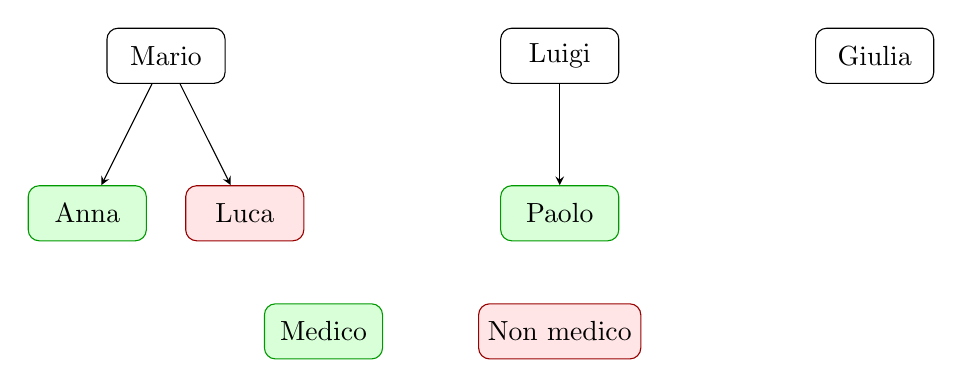
\begin{tikzpicture}[
    >=stealth,
    every node/.style={
        draw,
        rounded corners,
        minimum width=1.5cm,
        minimum height=0.7cm,
        align=center
    },
    medico/.style={fill=green!15,draw=green!60!black},
    nonmedico/.style={fill=red!10,draw=red!60!black}
]

% Genitori
\node (mario) at (0,2) {Mario};
\node (luigi) at (5,2) {Luigi};
\node (giulia) at (9,2) {Giulia};

% Figli
\node[medico] (anna) at (-1,0) {Anna};
\node[nonmedico] (luca) at (1,0) {Luca};
\node[medico] (paolo) at (5,0) {Paolo};

% Relazioni
\draw[->] (mario) -- (anna);
\draw[->] (mario) -- (luca);
\draw[->] (luigi) -- (paolo);

% Legenda
\node[medico] at (2,-1.5) {Medico};
\node[nonmedico] at (5,-1.5) {Non medico};

\end{tikzpicture}
\end{center}

\textbf{Quantificatore esistenziale: $\exists R.C$}

Consideriamo l'insieme:

\[
(\exists R.C)^{\mathcal I}
=
\left\{
d\in\Delta^{\mathcal I}
\mid
\exists e\in\Delta^{\mathcal I},
(d,e)\in R^{\mathcal I}
\land e\in C^{\mathcal I}
\right\}
\]
\[
\boxed{
(\exists R.C)^{\mathcal I}
=
\{Mario,Luigi\}
}
\]

\textbf{Quantificatore universale: $\forall R.C$}

Consideriamo l'insieme:

\[
(\forall R.C)^{\mathcal I}
=
\left\{
d\in\Delta^{\mathcal I}
\mid
\forall e\in\Delta^{\mathcal I},
(d,e)\in R^{\mathcal I}
\Rightarrow e\in C^{\mathcal I}
\right\}
\]

Analizziamo il caso di Mario, fissando $d=Mario$.

\begin{itemize}
    \item \textbf{Prima verifica: $e=Anna$.}

    \[
    \underbrace{(Mario,Anna)\in R^{\mathcal I}}_{\text{Vero}}
    \Rightarrow
    \underbrace{Anna\in C^{\mathcal I}}_{\text{Vero}}
    \]

    L'implicazione è vera.

    \item \textbf{Seconda verifica: $e=Luca$.}

    \[
    \underbrace{(Mario,Luca)\in R^{\mathcal I}}_{\text{Vero}}
    \Rightarrow
    \underbrace{Luca\in C^{\mathcal I}}_{\text{Falso}}
    \]

    L'implicazione è falsa.
\end{itemize}

Poiché il quantificatore è universale, la condizione
deve essere vera per ogni individuo $e$ del dominio.

È sufficiente una sola implicazione falsa per escludere Mario:

\[
Mario\notin(\forall R.C)^{\mathcal I}
\]

Consideriamo ora gli altri individui:
\end{example}

\begin{example}{Continuo}
\begin{itemize}
    \item \textbf{Luigi}: il suo unico collegamento tramite
    $R$ è verso Paolo, che appartiene a $C^{\mathcal I}$.
    Pertanto soddisfa la condizione universale.

    \item \textbf{Giulia}: non possiede collegamenti tramite
    $R$. L'implicazione è sempre vera per
    \textbf{verità vacua}.

    \item \textbf{Anna, Luca e Paolo}: non possiedono
    collegamenti tramite $R$ e soddisfano anch'essi
    la condizione per verità vacua.
\end{itemize}

Otteniamo quindi:

\[
\boxed{
(\forall R.C)^{\mathcal I}
=
\{Luigi,Giulia,Anna,Luca,Paolo\}
}
\]

\textbf{Conclusione.}

Il quantificatore esistenziale richiede almeno un
collegamento verso un individuo appartenente a $C$.

Il quantificatore universale richiede invece che tutti
i collegamenti esistenti tramite $R$ conducano a individui
appartenenti a $C$, ammettendo anche l'assenza
di collegamenti per verità vacua.

\end{example}


\section{Come leggere i nomi delle Logiche Descrittive}

I nomi delle DL sono acronimi che indicano quali «strumenti» o operatori
la logica possiede.

\begin{center}
    \begingroup
    \renewcommand{\arraystretch}{1.3}
    \begin{tabularx}{\linewidth}{@{}lX@{}}
        \hline
        \textbf{Nome} & \textbf{Strumenti o operatori} \\
        \hline
        \(\mathcal{ALC}\) & È la logica attributiva di base con complemento.
            Include \(\top,\bot\), concetti atomici, \(\sqcap,\sqcup,\neg\),
            \(\exists P.C,\forall P.C\) e assiomi GCI + ABox. \\
        \(\mathcal S\) & È l'abbreviazione per \(\mathcal{ALC}\) estesa con
            i \textbf{ruoli transitivi} (\(\operatorname{trans}(R)\)). \\
        \(\mathcal H\) & Aggiunge le \textbf{gerarchie di ruoli} (\(R\sqsubseteq R'\)). \\
        \(\mathcal O\) & Aggiunge i \textbf{nominali} (\(\{a\}\)). \\
        \(\mathcal I\) & Aggiunge i \textbf{ruoli inversi} (\(R^{-}\)). \\
        \(\mathcal Q\) & Aggiunge le \textbf{restrizioni numeriche qualificate}
            (\((\geq n\,R.C)\), \((\leq n\,R.C)\)). \\
        \(\mathcal N\) & Aggiunge le \textbf{restrizioni numeriche non qualificate}
            (\((\geq n\,R.\top)\), \((\leq n\,R.\top)\)). \\
        \hline
    \end{tabularx}
    \endgroup
\end{center}

\begin{observation}{Combinazioni chiave da ricordare per l'esame}
    \begin{itemize}
        \item \(\mathcal{ALCIO}\): logica \(\mathcal{ALC}\) + nominali
            (\(\mathcal O\)) + ruoli inversi (\(\mathcal I\)).
        \item \(\mathcal{SHOIN}\): è il fondamento matematico dello standard
            \textbf{OWL-DL} (\(\mathcal S+\mathcal H+\mathcal O+\mathcal I+\mathcal N\)).
        \item \(\mathcal{SROIQ}\): è il fondamento matematico dello standard
            \textbf{OWL~2-DL} (\(\mathcal S+\mathcal R+\mathcal O+\mathcal I+\mathcal Q\),
            con composizione di ruoli ristretta \(R_1\circ\cdots\circ R_n\sqsubseteq R\),
            il concetto \(\mathsf{Self}\) e il ruolo universale \(U\)).
    \end{itemize}
\end{observation}

\newpage

\section{Logiche Descrittive: leggere i grafi e interpretare le formule}

Questi esempi collegano i grafi alle definizioni di \textbf{dominio},
\textbf{interpretazione}, \textbf{concetto} e \textbf{ruolo}.

\subsection{Come leggere questi grafi}

Un \textbf{nodo} rappresenta un elemento del dominio \(\Delta^{\mathcal I}\).
Le etichette che assegniamo ai nodi servono a identificarli.

Una lettera come \(A\) o \(B\) accanto a un nodo indica
l'\textbf{appartenenza a un concetto}. Se il nodo \(d\) è etichettato con \(A\), allora:
\[
    d\in A^{\mathcal I}.
\]
Una \textbf{freccia} etichettata con \(R\), che parte da \(d\) e arriva a \(e\),
rappresenta una coppia appartenente al ruolo:
\[
    (d,e)\in R^{\mathcal I}.
\]
Chiamiamo \(e\) un \textbf{successore} di \(d\) tramite \(R\): è semplicemente
un nodo raggiunto da \(d\) seguendo una freccia \(R\) in uscita.

\begin{observation}{Che cosa significa valutare un concetto?}
    Un'espressione come \(\exists R.A\) descrive una categoria di elementi.
    La sua interpretazione \((\exists R.A)^{\mathcal I}\) è \textbf{l'insieme
    di tutti i nodi del grafo che soddisfano quella descrizione}.

    Per trovarlo, controlliamo ogni nodo e raccogliamo quelli che rispettano
    la condizione.
\end{observation}

\subsection{Primo grafo: restrizioni esistenziali e universali}

Nel primo disegno i nodi non hanno nomi. Per poterli indicare nelle
spiegazioni, li etichettiamo con \(x_1,\ldots,x_6\).

\begin{center}
    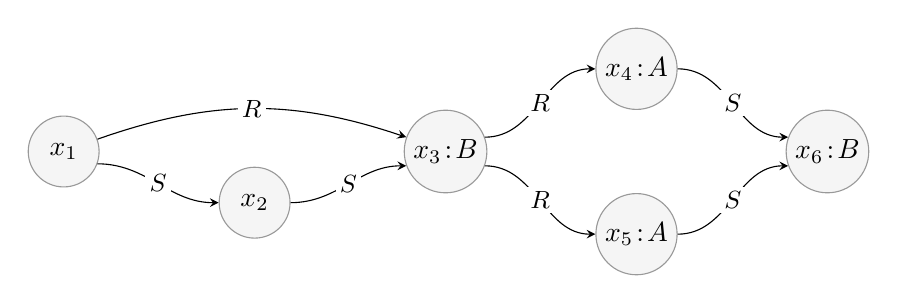
\begin{tikzpicture}[
        x=0.20\linewidth, y=1cm, >=stealth,
        vertice/.style={circle, draw=black!40, fill=black!4,
                        minimum size=9mm, inner sep=2pt},
        ruolo/.style={fill=white, inner sep=1.5pt, font=\small}
    ]
        \node[vertice] (x1) at (0,0)      {\(x_1\)};
        \node[vertice] (x2) at (1,-0.65)  {\(x_2\)};
        \node[vertice] (x3) at (2,0)      {\(x_3\!:\!B\)};
        \node[vertice] (x4) at (3,1.05)   {\(x_4\!:\!A\)};
        \node[vertice] (x5) at (3,-1.05)  {\(x_5\!:\!A\)};
        \node[vertice] (x6) at (4,0)      {\(x_6\!:\!B\)};

        \draw[->] (x1.20) to[bend left=19] node[ruolo] {\(R\)} (x3.160);
        \draw[->] (x1.-20) to[out=0,in=180] node[ruolo] {\(S\)} (x2.west);
        \draw[->] (x2.east) to[out=0,in=180] node[ruolo] {\(S\)} (x3.200);
        \draw[->] (x3.20) to[out=0,in=180] node[ruolo] {\(R\)} (x4.west);
        \draw[->] (x3.-20) to[out=0,in=180] node[ruolo] {\(R\)} (x5.west);
        \draw[->] (x4.east) to[out=0,in=180] node[ruolo] {\(S\)} (x6.160);
        \draw[->] (x5.east) to[out=0,in=180] node[ruolo] {\(S\)} (x6.200);
    \end{tikzpicture}
\end{center}

\subsubsection{L'interpretazione rappresentata dal grafo}

Il \textbf{dominio} contiene i sei nodi:
\[
    \Delta^{\mathcal I}=\{x_1,x_2,x_3,x_4,x_5,x_6\}.
\]
La funzione di interpretazione associa ai \textbf{concetti} questi insiemi:
\[
    A^{\mathcal I}=\{x_4,x_5\}
    \qquad
    B^{\mathcal I}=\{x_3,x_6\}.
\]
Ai \textbf{ruoli} associa gli insiemi delle coppie collegate dalle frecce:
\begin{gather*}
    R^{\mathcal I}=\{(x_1,x_3),(x_3,x_4),(x_3,x_5)\},\\
    S^{\mathcal I}=\{(x_1,x_2),(x_2,x_3),(x_4,x_6),(x_5,x_6)\}.
\end{gather*}

\newpage

\subsubsection{Un passaggio tramite \(S\): \(\exists S.B\)}

Il nodo \(x_2\) ha una freccia \(S\) che arriva a \(x_3\), e \(x_3\)
appartiene a \(B\). Quindi:
\[
    x_2\in(\exists S.B)^{\mathcal I}.
\]
Significa: \textbf{da \(x_2\) posso raggiungere almeno un elemento di \(B\)
seguendo una freccia \(S\)}. Anche \(x_4\) e \(x_5\) soddisfano questa
condizione, perché hanno una freccia \(S\) verso \(x_6\), che appartiene a \(B\).

\subsubsection{Due passaggi tramite $S$: $\exists S.\exists S.B$}

Consideriamo l'espressione:

\[
\exists S.\exists S.B
\]

Per comprenderne il significato, è importante ricordare che
$\exists S.B$ rappresenta esso stesso un \textbf{concetto},
ottenuto applicando il costruttore esistenziale $\exists S$
al concetto $B$.

Possiamo quindi riscrivere l'espressione, esplicitando
le parentesi:

\[
\exists S.(\exists S.B)
\]

La struttura è dunque della forma:

\[
\exists S.\underbrace{(\exists S.B)}_{\text{Nuovo concetto}}
\]

Questo significa che il costruttore esistenziale più esterno
viene applicato al concetto costruito dall'espressione interna.

\paragraph{Interpretazione semantica.}

Per comprendere quali individui appartengono al concetto
$\exists S.\exists S.B$, procediamo dall'interno verso l'esterno.

\begin{enumerate}
    \item \textbf{Primo passaggio: interpretazione di $\exists S.B$.}

    Consideriamo inizialmente il concetto più interno, lo consideriamo in modo semantico, cioè vediamo la sua definizione:

    \[
    (\exists S.B)^{\mathcal I}
    =
    \left\{
    e\in\Delta^{\mathcal I}
    \mid
    \exists f\in\Delta^{\mathcal I},
    (e,f)\in S^{\mathcal I}
    \land f\in B^{\mathcal I}
    \right\}
    \]

    Questo insieme contiene tutti gli individui $e$ che,
    attraverso la relazione $S$, sono collegati
    \textbf{ad almeno un individuo appartenente a $B$}.

    L'espressione $\exists S.B$ definisce quindi un nuovo
    concetto, la cui estensione è l'insieme appena costruito.

    \item \textbf{Secondo passaggio: interpretazione di
    $\exists S.(\exists S.B)$.}

    Applichiamo ora il costruttore esistenziale $\exists S$
    al concetto ottenuto nel passaggio precedente:

    \[
    (\exists S.(\exists S.B))^{\mathcal I}
    =
    \left\{
    d\in\Delta^{\mathcal I}
    \mid
    \exists e\in\Delta^{\mathcal I},
    (d,e)\in S^{\mathcal I}
    \land
    e\in(\exists S.B)^{\mathcal I}
    \right\}
    \]

    Questa volta cerchiamo gli individui $d$ che,
    attraverso la relazione $S$, sono collegati
    \textbf{ad almeno un individuo $e$ appartenente
    al concetto $\exists S.B$}.

    In altre parole, cerchiamo gli individui $d$
    che possono raggiungere un individuo appartenente
    a $B$ attraverso due collegamenti consecutivi
    tramite la relazione $S$.
\end{enumerate}

\paragraph{Interpretazione complessiva.}

Sostituendo la definizione del concetto interno
nella formula esterna, otteniamo:

\[
\boxed{
\begin{aligned}
(\exists S.\exists S.B)^{\mathcal I}
=
\bigl\{
d\in\Delta^{\mathcal I}
\mid {}&
\exists e,f\in\Delta^{\mathcal I}:\\
& (d,e)\in S^{\mathcal I}
\land (e,f)\in S^{\mathcal I}
\land f\in B^{\mathcal I}
\bigr\}
\end{aligned}
}
\]

Pertanto, un individuo $d$ appartiene al concetto
$\exists S.\exists S.B$ se esistono due individui $e$ e $f$
tali che:

\[
d\xrightarrow{S}e\xrightarrow{S}f
\qquad\text{con}\qquad f\in B^{\mathcal I}.
\]

\begin{observation}{Ordine di interpretazione dei concetti annidati}
    Quando abbiamo più costruttori annidati,
    possiamo interpretare l'espressione
    \textbf{dall'interno verso l'esterno}.

    Prima determiniamo l'estensione del concetto
    più interno, poi utilizziamo tale estensione
    per interpretare il concetto più esterno.

    Nel nostro caso, $\exists S.B$ individua
    gli elementi che raggiungono direttamente
    almeno un elemento di $B$ tramite $S$.

    Successivamente, $\exists S.(\exists S.B)$
    individua gli elementi che raggiungono tramite $S$
    almeno uno degli elementi individuati
    nel passaggio precedente.

    Di conseguenza, l'espressione descrive
    l'esistenza di un percorso formato da
    \textbf{due collegamenti consecutivi tramite $S$},
    che termina in un individuo appartenente a $B$.
\end{observation}
Partendo da \(x_1\) possiamo seguire questo percorso:
\[
    x_1\xrightarrow{S}x_2\xrightarrow{S}x_3.
\]
Il nodo finale \(x_3\) appartiene a \(B\). Quindi:
\[
    x_1\in(\exists S.\exists S.B)^{\mathcal I}.
\]
L'espressione richiede \textbf{un primo passaggio tramite \(S\) e poi un
secondo passaggio tramite \(S\), fino a un elemento di \(B\)}. Non richiede
che il nodo intermedio appartenga a \(B\).

Ricordati che la differenza principale è che:
\[
(\exists S.(\exists S.B))
\]
Esprime il concetto, in modo teorico, cioè si sta esprimendo che quello è un concetto non atomico
\\
Invece
\[
(\exists S.(\exists S.B))^{\mathcal I}
\]
Indica la sua definizione semantica matematica.


\subsubsection{Combinare più condizioni: \(\exists R.(B\sqcap\forall R.A)\)}

Consideriamo il seguente concetto composto:

\[
\exists R.(B\sqcap\forall R.A)
\]

Per comprenderne il significato, analizziamo
l'espressione dall'interno verso l'esterno:

\begin{enumerate}
    \item \textbf{Quantificatore universale $\forall R.A$:}

    Il concetto $\forall R.A$ individua tutti gli individui
    che, se possiedono successori tramite la relazione $R$,
    allora tali successori devono necessariamente
    appartenere al concetto $A$.

    Si noti che vengono inclusi anche gli individui
    che non possiedono alcun successore tramite $R$,
    per il principio della \textbf{verità vacua}.

    \item \textbf{Intersezione $B\sqcap\forall R.A$:}

    L'intersezione restringe ulteriormente
    l'insieme individuato nel passaggio precedente.

    In particolare, vengono selezionati soltanto
    gli individui che soddisfano entrambe le condizioni:
    \begin{itemize}
        \item appartengono al concetto $B$;
        \item tutti i loro eventuali successori tramite $R$
        appartengono al concetto $A$.
    \end{itemize}

    Pertanto, il concetto $B\sqcap\forall R.A$
    individua tutti gli individui appartenenti a $B$
    che possiedono esclusivamente successori
    tramite $R$ appartenenti ad $A$.

    \item \textbf{Quantificatore esistenziale esterno
    $\exists R.(B\sqcap\forall R.A)$:}

    Infine, applichiamo il costruttore esistenziale
    $\exists R$ al concetto ottenuto nel passaggio
    precedente.

    Vengono quindi individuati tutti gli individui
    che possiedono \textbf{almeno un successore tramite $R$}
    appartenente al concetto $B\sqcap\forall R.A$.

    In altre parole, cerchiamo gli individui $d$
    che sono collegati tramite $R$ ad almeno
    un individuo $e$ tale che:
    \begin{itemize}
        \item $e$ appartiene al concetto $B$;
        \item tutti gli eventuali successori di $e$
        tramite $R$ appartengono al concetto $A$.
    \end{itemize}
\end{enumerate}

\paragraph{Interpretazione complessiva.}


Il nodo \(x_1\) soddisfa questa descrizione. Infatti, con una freccia \(R\)
raggiunge \(x_3\), che appartiene a \(B\). Da \(x_3\) partono due frecce
\(R\), verso \(x_4\) e \(x_5\), ed entrambi appartengono ad \(A\). Quindi:
\[
    x_1\in\bigl(\exists R.(B\sqcap\forall R.A)\bigr)^{\mathcal I}.
\]


\subsubsection{Un nodo senza frecce uscenti: \(\forall R.\bot\) e \(\forall S.\bot\)}

Dal nodo \(x_6\) non parte alcuna freccia \(R\) o \(S\). Quindi:
\[
    x_6\in(\forall R.\bot)^{\mathcal I}
    \qquad
    x_6\in(\forall S.\bot)^{\mathcal I}.
\]
Ricordiamo che \(\bot^{\mathcal I}=\varnothing\). La formula \(\forall R.\bot\)
richiede che tutti i successori tramite \(R\) appartengano all'insieme vuoto.
Poiché nessun elemento può appartenervi, questa condizione è soddisfatta
\textbf{solo se non esistono successori tramite \(R\)}.

\begin{warning}{La restrizione universale non impone l'esistenza}
    Se un nodo non ha successori tramite \(R\), allora soddisfa \(\forall R.C\)
    per qualsiasi concetto \(C\), anche per \(C=\bot\).

    Non ci sono successori che possano violare la condizione: è la
    \textbf{verità per vacuità}.
\end{warning}

\newpage


\subsection{Secondo grafo: contare tutti i successori o solo quelli in \(A\)}

Anche qui introduciamo etichette per distinguere i nodi. Nel grafo, \(y_2\)
e \(y_3\) appartengono ad \(A\), mentre \(y_1\) non vi appartiene.

\begin{center}
    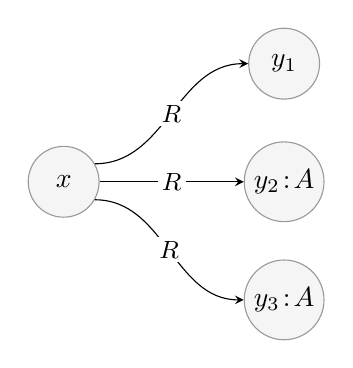
\begin{tikzpicture}[
        >=stealth,
        vertice/.style={circle, draw=black!40, fill=black!4,
                        minimum size=9mm, inner sep=2pt},
        ruolo/.style={fill=white, inner sep=1.5pt, font=\small}
    ]
        \node[vertice] (x)  at (0,0)      {\(x\)};
        \node[vertice] (y1) at (2.8,1.5)  {\(y_1\)};
        \node[vertice] (y2) at (2.8,0)    {\(y_2\!:\!A\)};
        \node[vertice] (y3) at (2.8,-1.5) {\(y_3\!:\!A\)};

        \draw[->] (x.30) to[out=0,in=180] node[ruolo] {\(R\)} (y1.west);
        \draw[->] (x.east) -- node[ruolo] {\(R\)} (y2.west);
        \draw[->] (x.-30) to[out=0,in=180] node[ruolo] {\(R\)} (y3.west);
    \end{tikzpicture}
\end{center}

L'interpretazione è:
\begin{gather*}
    \Delta^{\mathcal I}=\{x,y_1,y_2,y_3\}
    \qquad A^{\mathcal I}=\{y_2,y_3\},\\
    R^{\mathcal I}=\{(x,y_1),(x,y_2),(x,y_3)\}.
\end{gather*}

\subsubsection{Almeno tre successori: \((\geq 3\,R)\)}

Il nodo \(x\) ha tre successori distinti tramite \(R\): \(y_1\), \(y_2\)
e \(y_3\). Quindi:
\[
    x\in(\geq 3\,R)^{\mathcal I}.
\]
Qui \textbf{non imponiamo alcuna appartenenza a un concetto}. La scrittura
senza qualificazione è un'abbreviazione di:
\[
    (\geq 3\,R)\equiv(\geq 3\,R.\top).
\]
Poiché \(\top\) comprende tutti gli elementi del dominio, si contano tutti
i successori tramite \(R\).

\subsubsection{Almeno due successori in \(A\): \((\geq 2\,R.A)\)}

Dei tre successori di \(x\), solo \(y_2\) e \(y_3\) appartengono ad \(A\).
Quindi:
\[
    x\in(\geq 2\,R.A)^{\mathcal I}.
\]
Questa volta contiamo \textbf{solo i successori tramite \(R\) che appartengono
ad \(A\)}.

\subsubsection{Non almeno tre successori in \(A\): \(\neg(\geq 3\,R.A)\)}

I successori di \(x\) appartenenti ad \(A\) sono due, quindi non sono almeno tre:
\[
    x\in\bigl(\neg(\geq 3\,R.A)\bigr)^{\mathcal I}.
\]
Negare «almeno tre» significa dire \textbf{«al massimo due»}:
\[
    \neg(\geq 3\,R.A)\equiv(\leq 2\,R.A).
\]

\begin{observation}{Perché le tre condizioni della slide sono compatibili?}
    \(x\) ha \textbf{tre successori in totale}, ma \textbf{solo due
    appartengono ad \(A\)}.

    Soddisfa quindi contemporaneamente \((\geq 3\,R)\), \((\geq 2\,R.A)\)
    e \(\neg(\geq 3\,R.A)\). Le ultime due condizioni stabiliscono che i
    successori in \(A\) sono \textbf{esattamente due}.
\end{observation}

\subsection{Terzo grafo: calcolare gli insiemi descritti dalle formule}

Nelle ultime due slide i nodi hanno già le etichette \(d,e,f,g,b\).
Le manteniamo. I due disegni rappresentano \textbf{lo stesso grafo}.

\begin{center}
    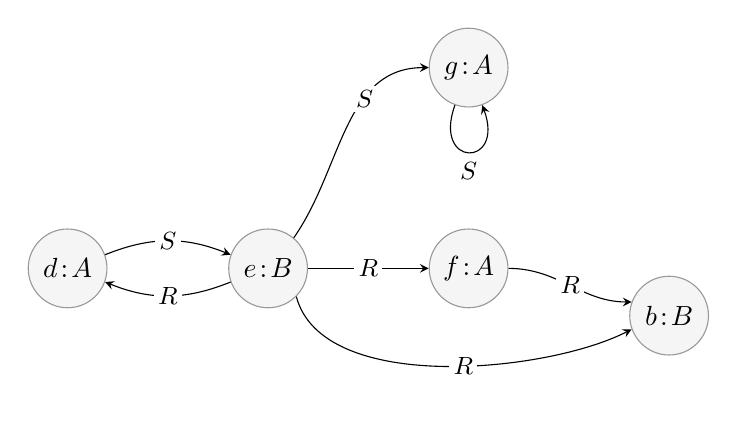
\begin{tikzpicture}[
        x=0.21\linewidth, y=1cm, >=stealth,
        vertice/.style={circle, draw=black!40, fill=black!4,
                        minimum size=10mm, inner sep=2pt},
        ruolo/.style={fill=white, inner sep=1.5pt, font=\small}
    ]
        \node[vertice] (d) at (0,0)     {\(d\!:\!A\)};
        \node[vertice] (e) at (1,0)     {\(e\!:\!B\)};
        \node[vertice] (f) at (2,0)     {\(f\!:\!A\)};
        \node[vertice] (g) at (2,2.55)  {\(g\!:\!A\)};
        \node[vertice] (b) at (3,-0.6)  {\(b\!:\!B\)};

        \draw[->] (d.20) to[bend left=22] node[ruolo] {\(S\)} (e.160);
        \draw[->] (e.200) to[bend left=22] node[ruolo] {\(R\)} (d.-20);
        \draw[->] (e.50) to[out=55,in=180] node[ruolo,pos=.65] {\(S\)} (g.west);
        \draw[->] (g.250) .. controls +(250:0.85cm) and +(290:0.85cm) ..
                  node[below,font=\small] {\(S\)} (g.290);
        \draw[->] (e.east) -- node[ruolo] {\(R\)} (f.west);
        \draw[->] (f.east) to[out=0,in=180] node[ruolo] {\(R\)} (b.160);
        \draw[->] (e.-45) .. controls +(0.13,-1.25) and +(-0.42,-0.55) ..
                  node[ruolo,pos=.55] {\(R\)} (b.200);
    \end{tikzpicture}
\end{center}

\subsubsection{Dominio, concetti e ruoli}

\begin{gather*}
    \Delta^{\mathcal I}=\{d,e,f,g,b\},\\
    A^{\mathcal I}=\{d,f,g\}
    \qquad B^{\mathcal I}=\{e,b\},\\
    R^{\mathcal I}=\{(e,d),(e,f),(e,b),(f,b)\},\\
    S^{\mathcal I}=\{(d,e),(e,g),(g,g)\}.
\end{gather*}
La coppia \((g,g)\) rappresenta \textbf{la freccia \(S\) che torna da \(g\)
a sé stesso}.

\subsubsection{Due passaggi tramite \(R\): \(\exists R.\exists R.\top\)}

Cerchiamo i nodi dai quali possiamo percorrere \textbf{due frecce \(R\)
consecutive}. Il punto di arrivo può essere qualsiasi elemento, perché
\(\top^{\mathcal I}=\Delta^{\mathcal I}\).

Nel grafo esiste questo percorso:
\[
    e\xrightarrow{R}f\xrightarrow{R}b.
\]
Nessun altro nodo permette due passaggi consecutivi tramite \(R\). Perciò:
\[
    (\exists R.\exists R.\top)^{\mathcal I}=\{e\}.
\]

\subsubsection{Esattamente un predecessore: \((=1\,R^{-})\)}

Il \textbf{ruolo inverso} inverte la direzione delle coppie:
\[
    (u,v)\in(R^{-})^{\mathcal I}\iff(v,u)\in R^{\mathcal I}.
\]
Quindi contare i successori tramite \(R^{-}\) equivale a contare
\textbf{i nodi da cui riceviamo una freccia \(R\)}.

Il nodo \(d\) riceve una freccia \(R\) solo da \(e\). Anche \(f\) riceve
una freccia \(R\) solo da \(e\). Invece, \(b\) ne riceve da due nodi
distinti, \(e\) e \(f\), mentre \(e\) e \(g\) non ne ricevono nessuna.
Quindi:
\[
    (=1\,R^{-})^{\mathcal I}=\{d,f\}.
\]

\subsubsection{Due passaggi tramite \(S\) fino ad \(A\): \(\exists S.\exists S.A\)}

Cerchiamo i nodi dai quali possiamo seguire \textbf{due frecce \(S\)
consecutive} e terminare in un nodo di \(A\).

I percorsi che soddisfano questa condizione sono:
\begin{gather*}
    d\xrightarrow{S}e\xrightarrow{S}g,\\
    e\xrightarrow{S}g\xrightarrow{S}g,\\
    g\xrightarrow{S}g\xrightarrow{S}g.
\end{gather*}
Il punto finale è sempre \(g\), che appartiene ad \(A\). Quindi:
\[
    (\exists S.\exists S.A)^{\mathcal I}=\{d,e,g\}.
\]

\begin{observation}{Si può attraversare più volte lo stesso nodo}
    Una catena esistenziale non richiede nodi tutti distinti. La freccia
    da \(g\) a sé stesso può essere percorsa due volte: per questo anche
    \(g\) soddisfa \(\exists S.\exists S.A\).
\end{observation}

\subsubsection{Tutti i successori tramite \(R\) in \(A\): \(\forall R.A\)}

Il nodo \(e\) \textbf{non soddisfa} la condizione: ha due successori in \(A\),
cioè \(d\) e \(f\), ma ha anche il successore \(b\), che non appartiene ad \(A\).

Nemmeno \(f\) la soddisfa, perché ha una freccia \(R\) verso \(b\).

I nodi \(d\), \(g\) e \(b\) \textbf{non hanno frecce \(R\) uscenti}.
Soddisfano quindi la condizione per vacuità:
\[
    (\forall R.A)^{\mathcal I}=\{d,g,b\}.
\]

\begin{warning}{Il concetto \(A\) riguarda i nodi raggiunti}
    \(\forall R.A\) non richiede che il nodo di partenza appartenga ad \(A\).
    Richiede che appartengano ad \(A\) tutti i suoi successori tramite \(R\).

    Per questo anche \(b\), che appartiene a \(B\), soddisfa la formula:
    non ha successori tramite \(R\) che possano violarla.
\end{warning}

\subsubsection{Un successore tramite \(S\) che soddisfa \(\forall R.A\): \(\exists S.\forall R.A\)}
Per comprenderne il significato, procediamo
\textbf{dall'interno verso l'esterno}, distinguendo due passaggi.

\begin{enumerate}
    \item \textbf{Primo passaggio: interpretazione di $\forall R.A$.}

    Individuiamo tutti gli individui del dominio che,
    attraverso la relazione $R$, sono collegati
    esclusivamente a individui appartenenti al concetto $A$.

    Formalmente:

    \[
    (\forall R.A)^{\mathcal I}
    =
    \left\{
    e\in\Delta^{\mathcal I}
    \mid
    \forall f\in\Delta^{\mathcal I},
    (e,f)\in R^{\mathcal I}
    \Rightarrow f\in A^{\mathcal I}
    \right\}
    \]

    Si noti che appartengono a questo insieme anche gli
    individui che non possiedono alcun successore tramite
    $R$, per il principio della \textbf{verità vacua}.

    \item \textbf{Secondo passaggio: interpretazione di
    $\exists S.(\forall R.A)$.}

    Una volta individuati gli elementi appartenenti
    al concetto $\forall R.A$, cerchiamo tutti gli
    individui del dominio che sono collegati tramite
    la relazione $S$ ad \textbf{almeno uno degli individui
    individuati nel passaggio precedente}.

    Formalmente:

    \[
    (\exists S.\forall R.A)^{\mathcal I}
    =
    \left\{
    d\in\Delta^{\mathcal I}
    \mid
    \exists e\in\Delta^{\mathcal I},
    (d,e)\in S^{\mathcal I}
    \land
    e\in(\forall R.A)^{\mathcal I}
    \right\}
    \]
\end{enumerate}

\subsubsection{Almeno tre successori tramite \(R\): \((\geq 3\,R)\)}

Il nodo \(e\) ha tre successori distinti tramite \(R\): \(d\), \(f\) e \(b\).

Il nodo \(f\) ne ha uno, mentre gli altri non ne hanno. Quindi:
\[
    (\geq 3\,R)^{\mathcal I}=\{e\}.
\]

\section{Calcolo}
\subsection{Struttura di una Knowledge Base (KB)}

\begin{definition}{Base di conoscenza}
    Una \textbf{base di conoscenza} (\emph{Knowledge Base}, KB) è un insieme
    finito di \textbf{assiomi}, cioè affermazioni che descrivono le regole di
    un determinato ambito.

    Queste informazioni si organizzano in tre parti: \textbf{TBox},
    \textbf{RBox} e \textbf{ABox}.
\end{definition}

\subsection{TBox (\emph{Terminological Box}): le regole sui concetti}

\begin{definition}{TBox e inclusioni generali di concetto}
    La \textbf{TBox} descrive le relazioni generali tra i concetti, cioè tra
    le categorie di oggetti. Contiene le \textbf{inclusioni generali di
    concetto} (GCI), che hanno la forma
    \[
        C\sqsubseteq D.
    \]
    Questa espressione significa che \textbf{ogni individuo che appartiene al
    concetto \(C\) appartiene anche al concetto \(D\)}.
\end{definition}

\begin{observation}{Esempio di inclusione di concetto}
    \[
        \mathsf{Studente}\sqsubseteq\mathsf{Persona}.
    \]
    Significa che \textbf{ogni studente è una persona}. È una regola generale
    che vale per tutti gli studenti.
\end{observation}

Dal punto di vista degli insiemi, in un'interpretazione \(\mathcal I\):
\[
    C^{\mathcal I}\subseteq D^{\mathcal I}.
\]

\subsection{RBox (\emph{Role Box}): le regole sulle relazioni}

\begin{definition}{RBox}
    La \textbf{RBox} descrive le proprietà dei ruoli, cioè delle relazioni tra
    individui. Può contenere:
    \begin{itemize}
        \item inclusioni di ruolo;
        \item dichiarazioni di funzionalità;
        \item transitività.
    \end{itemize}
\end{definition}

\subsubsection{Inclusioni di ruolo}

\begin{definition}{Inclusione di ruolo}
    Un'inclusione di ruolo ha la forma
    \[
        R\sqsubseteq R'.
    \]
    Significa che \textbf{ogni coppia di individui collegata da \(R\) è
    collegata anche da \(R'\)}.
\end{definition}
\begin{observation}{Esempio di inclusione di ruolo}
    \[
        \mathsf{haPadre}\sqsubseteq\mathsf{haGenitore}.
    \]
    Se Mario ha Luigi come padre, allora Mario ha Luigi anche come genitore.
\end{observation}

\subsubsection{Ruoli funzionali}

\begin{definition}{Funzionalità di un ruolo}
    La dichiarazione
    \[
        \operatorname{func}(R)
    \]
    stabilisce che \textbf{ogni individuo può essere collegato tramite \(R\)
    ad al massimo un individuo distinto}.
\end{definition}
\begin{observation}{Esempio di ruolo funzionale}
    \[
        \operatorname{func}(\mathsf{haMadreBiologica}).
    \]
    Significa che ogni individuo può avere \textbf{al massimo una madre biologica}.
\end{observation}
\begin{warning}{«Al massimo uno» non significa «esattamente uno»}
    La funzionalità impedisce di avere due individui distinti come destinazione
    dello stesso ruolo, ma \textbf{non impone che una relazione esista}.
\end{warning}


\subsubsection{Ruoli transitivi}

\begin{definition}{Transitività di un ruolo}
    La dichiarazione
    \[
        \operatorname{trans}(R)
    \]
    stabilisce che, se \(a\) è collegato a \(b\) tramite \(R\) e \(b\) è
    collegato a \(c\) tramite \(R\), allora anche \(a\) è collegato a \(c\)
    tramite \(R\):
    \[
        R(a,b)\land R(b,c)\ \Rightarrow\ R(a,c).
    \]
\end{definition}
\begin{observation}{Esempio di ruolo transitivo}
    Il ruolo \(\mathsf{haAntenato}\) è transitivo. Se Luigi è un antenato di
    Mario e Giovanni è un antenato di Luigi, allora \textbf{Giovanni è anche
    un antenato di Mario}. In OWL: \texttt{owl:TransitiveProperty}.
\end{observation}

\subsection{ABox (\emph{Assertion Box}): i fatti sui singoli individui}

\begin{definition}{ABox}
    La \textbf{ABox} contiene le \textbf{asserzioni}, cioè le affermazioni
    che riguardano individui specifici, come \(\mathsf{mario}\) o \(\mathsf{luigi}\).
\end{definition}

\subsubsection{Asserzioni di concetto}

\begin{definition}{Asserzione di concetto}
    Un'asserzione di concetto ha la forma
    \[
        C(a).
    \]
    Significa che \textbf{l'individuo \(a\) appartiene al concetto \(C\)}.
\end{definition}
\begin{observation}{Esempio di asserzione di concetto}
    \[
        \mathsf{Studente}(\mathsf{mario}).
    \]
    Questa affermazione dice che \textbf{Mario è uno studente}.
    In RDF: \texttt{rdf:type}.
\end{observation}

\subsubsection{Asserzioni di ruolo}

\begin{definition}{Asserzione di ruolo}
    Un'asserzione di ruolo ha la forma
    \[
        R(a,b).
    \]
    Significa che \textbf{l'individuo \(a\) è collegato all'individuo \(b\)
    tramite il ruolo \(R\)}.
\end{definition}
\begin{observation}{Esempio di asserzione di ruolo}
    \[
        \mathsf{haAmico}(\mathsf{mario},\mathsf{luigi}).
    \]
    Questa affermazione dice che \textbf{Mario ha Luigi come amico}.
\end{observation}

\begin{observation}{Come si usano insieme queste informazioni?}
    Nella \textbf{TBox} possiamo avere la regola generale
    \(\mathsf{Studente}\sqsubseteq\mathsf{Persona}\).

    Nella \textbf{ABox} possiamo avere il fatto \(\mathsf{Studente}(\mathsf{mario})\).

    Combinando queste informazioni, possiamo \textbf{dedurre che Mario è
    una persona}, cioè \(\mathsf{Persona}(\mathsf{mario})\).
\end{observation}
La Knowledge Base quindi \(\mathcal K\) contiene un insieme di assiomi che rappresentano le conoscenze che assumiamo vere sul dominio.
\textbf{Tuttavia, non è detto che questi assiomi siano veri in qualsiasi interpretazione.}


Infatti:
\begin{itemize}
    \item Se un'interpretazione \(\mathcal I\) soddisfa tutti gli assiomi della KB, allora è un modello della KB:
    \[
    \mathcal I\models\mathcal K
    \]
    (poi piu in la vedremo la definizione formale, per il momento ti basta sapere questo.)
    \item Se un'interpretazione non è un modello della KB:
    \[
\mathcal I\not\models\mathcal K
    \]
\end{itemize}
La KB specifica ciò che vogliamo sia vero (ma non tutti le interpretazioni possono soddisfare), mentre le interpretazioni rappresentano i possibili significati matematici dei simboli. I modelli sono precisamente quelle interpretazioni in cui tutti gli assiomi della KB risultano veri.

\begin{definition}{$Ax$}
    $Ax$ indica un \textbf{assioma generico}, cioè una formula logica che esprime una regola, un vincolo o un fatto.

    Ad esempio,$\mathsf{Vegetable}\sqsubseteq\mathsf{Food}$ è un'assioma che esprime la regola "Ogni verdura è un alimento".

    Tutte le inclusioni di ruolo, di concetto, o tutte le asserzioni di ruolo o di concetto, sono delle $Ax$.
\end{definition}


\begin{definition}{Modello di una KB, $\mathcal{I} \models KB$}
    Un'interpretazione $\mathcal{I}$ è detta \textbf{modello} di una
    Knowledge Base $KB$ se e solo se soddisfa ($\models$) tutti gli assiomi
    contenuti nella $KB$.

    Formalmente:
    \[
        \mathcal{I} \models KB
        \iff
        \forall Ax \in KB, \quad \mathcal{I} \models Ax.
    \]
\end{definition}


\begin{observation}{}
    Dire che un'interpretazione $\mathcal{I}$ soddisfa un assioma
    $Ax$, ossia
    \[
        \mathcal{I} \models Ax,
    \]
    significa che l'assioma $Ax$ risulta vero sotto l'interpretazione
    $\mathcal{I}$.

    Se tutti gli assiomi della $KB$ risultano veri sotto la stessa
    interpretazione $\mathcal{I}$, allora tale interpretazione
    è detta \textbf{modello della KB}.
\end{observation}


\begin{definition}{Conseguenza semantica, $KB \models Ax$ }
    Un assioma $Ax$ è detto \textbf{conseguenza semantica} di una
    Knowledge Base $KB$ se e solo se viene soddisfatto da tutti
    i possibili modelli della $KB$.

    Formalmente:
    \[
        KB \models Ax
        \iff
        \forall \mathcal{I}, \quad
        \mathcal{I} \models KB
        \implies
        \mathcal{I} \models Ax.
    \]
\end{definition}


\newpage
\subsubsection{Requisiti dei motori di inferenza (Inference Engines)}

\begin{observation}{}
\textbf{Inferire} significa ricavare una conclusione a partire dagli assiomi della KB, applicando una
regola di ragionamento.
\end{observation}

I software che effettuano ragionamenti sulle ontologie, detti
\textbf{reasoner} (o motori di inferenza), devono soddisfare due
proprietà fondamentali:

\begin{itemize}
    \item \textbf{Correttezza (Soundness):} il motore di inferenza
    deve inferire \textbf{solamente} gli assiomi che sono
    effettivamente conseguenze semantiche della $KB$.

    Formalmente:
    \[
        KB \vdash Ax \implies KB \models Ax.
    \]

    \item \textbf{Completezza (Completeness):} il motore di inferenza
    deve essere in grado di inferire \textbf{tutti} gli assiomi
    che sono conseguenze semantiche della $KB$.

    Formalmente:
    \[
        KB \models Ax \implies KB \vdash Ax.
    \]
\end{itemize}

Dove:
\begin{itemize}
    \item $KB \vdash Ax$ \textbf{indica che l'assioma $Ax$ è derivabile
    dalla $KB$ mediante il sistema di inferenza considerato;}
    \item $KB \models Ax$ indica che l'assioma $Ax$ è una
    conseguenza semantica della $KB$.
\end{itemize}

Pertanto, se un motore di inferenza è sia corretto sia completo,
allora vale la seguente equivalenza:
\[
    \boxed{KB \vdash Ax \iff KB \models Ax}
\]


\subsection{Vantaggio della riduzione dei reasoning tasks}
    Un reasoner ha il compito di risolvere diversi problemi di
    ragionamento, detti \textbf{reasoning tasks}.

    I reasoning tasks sono problemi di ragionamento che un reasoner deve risolvere a partire dalla conoscenza formalizzata in una Knowledge Base (\(KB\)).

    principalmente sono problemi che sono di conseguenza semantica, ovvero la "$KB$ è conseguenza semantica di un assioma?"

    Nelle logiche descrittive sufficientemente espressive,
    tuttavia, \textbf{i principali reasoning tasks possono essere
    ridotti l'uno all'altro}.

    Questa proprietà ci permette di sviluppare un reasoner
    che \textbf{implementa direttamente gli algoritmi risolutivi
    soltanto per alcuni task fondamentali}.

    Quando viene richiesto di risolvere un task per il quale
    non \textbf{è stato implementato un algoritmo risolutivo specifico,
    è sufficiente ricondurlo, mediante un'opportuna riduzione,
    a un task che il reasoner è già in grado di risolvere}.

    \textbf{Il vantaggio consiste quindi nel fatto che non è
    necessario progettare un algoritmo risolutivo specifico
    per ciascun reasoning task, ma è possibile concentrare
    gli sforzi sull'implementazione e sull'ottimizzazione
    di pochi algoritmi fondamentali.}



\newpage
\subsubsection{Principali Reasoning Task}
I principali reasoning task, di cui abbiamo accenato anche prima, sono principalmente:


\begin{table}[htbp]
    \centering
    \renewcommand{\arraystretch}{1.8}
    \begin{tabular}{|p{0.27\textwidth}|p{0.24\textwidth}|p{0.39\textwidth}|}
        \hline
        \textbf{Reasoning Task} &
        \textbf{Formula logica} &
        \textbf{Definizione semantica} \\
        \hline

        \textbf{1. Sussunzione}
        \newline
        \textit{(Subsumption)}
        &
        $KB \models C \sqsubseteq D$?
        &
        $\displaystyle
        \forall \mathcal{I}, \quad
        \mathcal{I} \models KB
        \implies
        C^{\mathcal{I}} \subseteq D^{\mathcal{I}}$
        \\
        \hline

        \textbf{2. Coerenza della KB}
        \newline
        \textit{(KB Consistency)}
        &
        $KB \not\models \top \sqsubseteq \bot$?
        &
        $\displaystyle
        \exists \mathcal{I} :
        \mathcal{I} \models KB$
        \\
        \hline

        \textbf{3. Coerenza del concetto}
        \newline
        \textit{(Concept Consistency / Satisfiability)}
        &
        $KB \not\models C \sqsubseteq \bot$?
        &
        $\displaystyle
        \exists \mathcal{I} :
        \mathcal{I} \models KB
        \land
        C^{\mathcal{I}} \neq \emptyset$
        \\
        \hline

        \textbf{4. Controllo di istanza}
        \newline
        \textit{(Instance Checking)}
        &
        $KB \models C(a)$?
        \newline
        oppure
        \newline
        $KB \models R(a,b)$?
        &
        $\displaystyle
        \forall \mathcal{I}, \quad
        \mathcal{I} \models KB
        \implies
        a^{\mathcal{I}} \in C^{\mathcal{I}}$
        \newline
        oppure
        \newline
        $\displaystyle
        \forall \mathcal{I}, \quad
        \mathcal{I} \models KB
        \implies
        (a^{\mathcal{I}},b^{\mathcal{I}})
        \in R^{\mathcal{I}}$
        \\
        \hline
    \end{tabular}
    \caption{Principali reasoning tasks e relative definizioni semantiche.}
    \label{tab:reasoning_tasks}
\end{table}

\begin{observation}
    Per ottenere la definizione semantica, quello che si fa è (considero la prima, poi il procedimento è uguale):
    \[
KB\models C\sqsubseteq D.
\]

Per definizione di conseguenza semantica:
\[
\iff
\forall\mathcal I,\quad
(\mathcal I\models KB\implies
\mathcal I\models C\sqsubseteq D).
\]

Tuttavia, grazie alla definizione di soddisfazione, sappiamo che:
\[
\mathcal I\models C\sqsubseteq D
\iff
C^{\mathcal I}\subseteq D^{\mathcal I}.
\]
\end{observation}

\subsubsection{I meccanismi di riduzione}
La riduzione si basa su precise equivalenze logiche. Di seguito sono illustrati i passaggi
fondamentali, per la riduzione fra i 4 problemi principali. 
\paragraph{Da Sussunzione a Coerenza del Concetto}
L'idea è che vogliamo risolvere il task di sussunzione, ma senza utilizzare direttamente un algoritmo di sussunzione. Vogliamo invece sfruttare un algoritmo che sappia già risolvere il task di soddisfacibilità di un concetto (Concept Satisfiability)
\begin{observation}{}
    Per questa riduzione, useremo una regola che conosciamo dalla teoria degli insiemi, cioè
    \[
    A \subseteq B \Leftrightarrow A \cup \neg B = \emptyset
    \]
    Cioè questo significa:
    \begin{enumerate}
        \item Il membro a sinistra significa che ogni elemento di $A$ appartiene anche a $B$.
        \item Il membro di destra identifica solo gli elementi di A e non di B, quindi gli elementi esclusivamente di $A$, questo deve essere vuoto, perchè se sono sottoinsiemi, $A$ non deve avere nessun elemento esclusivo.
    \end{enumerate}
\end{observation}
Quindi supponiamo che ci viene dato il seguente task
\[
KB\models C\sqsubseteq D.
\]

Dalla definizione di conseguenza semantica sappiamo che ciò equivale a verificare:
\[
\forall\mathcal I,\quad
\mathcal I\models KB
\implies C^{\mathcal I}\subseteq D^{\mathcal I}.
\]

pplicando la semantica formale dell'intersezione, otteniamo:
\[
\boxed{
C^{\mathcal I}\subseteq D^{\mathcal I}
\iff
(C\sqcap\neg D)^{\mathcal I}=\emptyset
}
\]

Applicando la definizione semantica:
\[
\iff
\forall\mathcal I,\quad
\mathcal I\models KB
\implies C^{\mathcal I}\subseteq D^{\mathcal I}
\]

Utilizzando l'equivalenza insiemistica appena vista:
\[
\iff
\forall\mathcal I,\quad
\mathcal I\models KB
\implies(C\sqcap\neg D)^{\mathcal I}=\emptyset
\]

Ciò equivale a dire che non esiste alcun modello della \(KB\) nel quale il concetto \(C\sqcap\neg D\) sia non vuoto:
\[
\iff
\neg\exists\mathcal I:
\bigl(\mathcal I\models KB
\land
(C\sqcap\neg D)^{\mathcal I}\neq\emptyset\bigr).
\]

Ma questa è esattamente la negazione della definizione di soddisfacibilità di un concetto rispetto alla \(KB\).

Abbiamo quindi ottenuto la regola di riduzione:
\[
\boxed{
KB\models C\sqsubseteq D
\iff
KB\models(C\sqcap\neg D)\sqsubseteq\bot
}
\]

\newpage

\paragraph{Riduzione da coerenza del concetto a coerenza della KB}
L'idea alla base della riduzione è che io voglio risolvere un compito di coerenza del concetto, avendo a disposizione un algoritmo di coerenza della $KB$


Supponiamo di voler verificare se un concetto $C$ è coerente
rispetto a una Knowledge Base $KB$ (quindi ci viene dato questo task in input insomma), ossia per definizione:
\[
    KB \not\models C \sqsubseteq \bot.
\]

Dalla definizione semantica di coerenza di un concetto, sappiamo
che ciò equivale a verificare se:
\[
    \exists \mathcal{I} :
    \bigl(\mathcal{I} \models KB
    \land C^{\mathcal{I}} \neq \emptyset\bigr).
\]

Quindi Il nostro obiettivo iniziale è verificare la coerenza del concetto \(C\) rispetto alla \(KB\), ossia:
\[
\exists\mathcal I:
\underbrace{\mathcal I\models KB}_{\text{Prima condizione}}
\land
\underbrace{C^{\mathcal I}\neq\emptyset}_{\text{Seconda condizione}}.
\]

Quindi dobbiamo trovare un'interpretazione che soddisfi contemporaneamente due condizioni.

Però noi abbiamo a disposizione solo un reasoner che sappia risolvere solamente il task di coerenza della KB.

Questo reasoner è in grado di verificare:
\[
\exists\mathcal I:\mathcal I\models KB.
\]

Cioè il reasoner ci sa solo dire se una $KB$ è coerente.

L'idea alla base della riduzione è quella di costruire una nuova Knowledge Base:
\[
    KB' = KB \cup
    \{\top \sqsubseteq \exists R_{\mathrm{new}}.C\},
\]
dove $R_{\mathrm{new}}$ è un nuovo nome di ruolo, non presente
né nella $KB$ originale né nel concetto $C$.

Il nuovo assioma è \textbf{un'assioma di inclusione di ruolo}:
\[
    \top \sqsubseteq \exists R_{\mathrm{new}}.C
\]
impone che ogni elemento del dominio sia collegato, attraverso
il ruolo $R_{\mathrm{new}}$, ad almeno un elemento appartenente
al concetto $C$.

Applicando la definizione che un interpretazione deve essere un modello rispetto alla $KB'$ si ha che ogni assioma della nuova Knowledge Base deve essere vero nell'interpretazione, otteniamo quindi quando si arriva al nuovo assioma:
\[
    \mathcal{I} \models
    \top \sqsubseteq \exists R_{\mathrm{new}}.C
    \iff
    \forall x \in \Delta^{\mathcal{I}}, \quad
    \exists y \in C^{\mathcal{I}} :
    (x,y) \in R_{\mathrm{new}}^{\mathcal{I}}.
\]

Poiché, per definizione di interpretazione, il dominio
$\Delta^{\mathcal{I}}$ è sempre non vuoto, affinché questo
assioma possa essere soddisfatto deve necessariamente valere:
\[
    C^{\mathcal{I}} \neq \emptyset.
\]

Quindi abbiamo trasformato il task iniziare, di coerenza del concetto, dove devo verificare due principali condizioni, in un task dove devo verificare la coerenza di una nuova $KB'$, che esattamente quello che il mio reasoner sa fare
\[
\exists\mathcal I:\mathcal I\models KB'.
\]
e se so verificare questo, allora ho risolto il mio problema originale, soddisfando entrambe le condizioni.

\newpage
\paragraph{Riduzione da Coerenza della KB a Instance Checking}
L'idea alla base di questa riduzione è che voglio risolvere un problema di Coerenza dell KB, avendo però a disposizione un algoritmo
di Instance Checking.

Supponiamo di voler verificare se una Knowledge Base $KB$
è coerente, ossia se:
\[
    KB \not\models \top \sqsubseteq \bot.
\]

Dalla definizione semantica di coerenza della KB, sappiamo
che ciò equivale a verificare se esiste almeno un modello
della $KB$:
\[
    \exists \mathcal{I} : \mathcal{I} \models KB.
\]

Supponiamo, tuttavia, di avere a disposizione solamente
un algoritmo in grado di risolvere il task di controllo
di istanza (\textit{Instance Checking}).

L'idea alla base della riduzione consiste nello sfruttare
il fatto che, per definizione di semantica formale,
il concetto $\bot$ viene sempre interpretato come
l'insieme vuoto:
\[
    \forall \mathcal{I}, \quad
    \bot^{\mathcal{I}} = \emptyset.
\]

Consideriamo quindi un generico nome di individuo $a$
(eventualmente introdotto appositamente) e chiediamoci
se l'asserzione $\bot(a)$ sia una conseguenza semantica
della $KB$:
\[
    KB \models \bot(a).
\]

Dalla definizione semantica del task di controllo di
istanza, sappiamo che:
\[
    KB \models \bot(a)
    \iff
    \forall \mathcal{I}, \quad
    \bigl(\mathcal{I} \models KB
    \implies
    a^{\mathcal{I}} \in \bot^{\mathcal{I}}\bigr).
\]

Poiché $\bot^{\mathcal{I}} = \emptyset$, otteniamo:
\[
    KB \models \bot(a)
    \iff
    \forall \mathcal{I}, \quad
    \bigl(\mathcal{I} \models KB
    \implies
    a^{\mathcal{I}} \in \emptyset\bigr).
\]

Tuttavia, nessun elemento può appartenere all'insieme
vuoto. Il conseguente dell'implicazione è quindi
\textbf{sempre falso}.

Ricordando la seguente equivalenza logica:
\[
    (P \implies \mathrm{False}) \iff \neg P,
\]
otteniamo:
\[
    KB \models \bot(a)
    \iff
    \forall \mathcal{I}, \quad
    \mathcal{I} \not\models KB.
\]

Applicando le proprietà dei quantificatori:
\[
    KB \models \bot(a)
    \iff
    \neg \exists \mathcal{I} :
    \mathcal{I} \models KB.
\]

Abbiamo quindi ottenuto esattamente la definizione
semantica di incoerenza della $KB$.

Negando entrambi i membri dell'equivalenza, otteniamo:
\[
    KB \not\models \bot(a)
    \iff
    \exists \mathcal{I} :
    \mathcal{I} \models KB.
\]

Riconosciamo, nel membro di destra, la definizione
semantica di coerenza della $KB$.

\medskip
\textbf{Regola di riduzione.}

Possiamo quindi esprimere la riduzione mediante la
seguente equivalenza:
\[
    \boxed{
        KB \not\models \top \sqsubseteq \bot
        \iff
        KB \not\models \bot(a)
    }
\]

Quindi verificare la Coerenza della $KB$ può essere fatto medianete un task di Instance Checking.

\paragraph{Riduzione di tutti i task alla Sussunzione}
Sappi che tutti i task fondamentali visti prima possono essere ridotti alla Sussunzione.

\newpage
\subsection{Tautologie}
Nelle Logiche Descrittive (DL) è importante distinguere due
concetti fondamentali:
\begin{itemize}
    \item Le \textbf{tautologie}, ossia formule logiche che
    risultano vere in qualsiasi interpretazione possibile,
    indipendentemente dagli assiomi presenti nella $KB$.

    \item Le \textbf{regole di derivazione}, ossia regole logiche
    che permettono di ricavare nuove conclusioni a partire da
    determinate premesse.
    Le regole di derivazione permettono di inferire.
    I reasoner possono sfruttare tali regole per inferire
    conoscenza implicitamente contenuta nella $KB$.
\end{itemize}

\begin{observation}{}
    Le regole di derivazione e i reasoning tasks sono due concetti distinti, ma strettamente collegati.
    \begin{enumerate}
        \item I reasoning tasks rappresentano i problemi di ragionamento che il reasoner deve risolvere a partire da una \(KB\).
        \item Le regole di derivazione rappresentano gli strumenti logici che il reasoner può utilizzare per inferire nuova conoscenza e, quindi, per risolvere i reasoning tasks.
    \end{enumerate}
    In altre parole, il reasoning task rappresenta che cosa vogliamo verificare, mentre le regole di derivazione rappresentano uno dei modi attraverso cui possiamo ottenere la risposta.
    Comunque tieni conto che noi prima abbiamo visto meccanismi di riduzione, ma il task a cui ci riduciamo comunque deve essere risolto.
    Supponiamo di avere la seguente Knowledge Base:
    \[
    KB=\{A\sqsubseteq B,\ B\sqsubseteq C\}.
    \]

    Il reasoning task che vogliamo risolvere è quello di sussunzione:
    \[
    KB\models A\sqsubseteq C\;?
    \]
    E quindi per risolverlo useremo delle regole di derivazione, partendo appunto dalla $KB$.
\end{observation}

\subsection{Tautologie nelle Logiche Descrittive}

\begin{definition}{Tautologia}
    Una \textbf{tautologia} è un assioma $Ax$ che viene
    soddisfatto da qualsiasi interpretazione $\mathcal{I}$,
    indipendentemente dalla Knowledge Base considerata.
    Cioè è vero in ogni interpretazione.

    Formalmente, un assioma $Ax$ è una tautologia se e solo se:
    \[
        \forall \mathcal{I}, \quad \mathcal{I} \models Ax.
    \]

    Per indicare che un assioma è una tautologia, possiamo
    utilizzare la seguente notazione:
    \[
        \models Ax.
    \]
\end{definition}

\begin{observation}{Differenza tra tautologia e conseguenza semantica}
    Non bisogna confondere il concetto di tautologia con
    quello di conseguenza semantica di una $KB$.

    Infatti:
    \begin{itemize}
        \item $KB \models Ax$ significa che l'assioma $Ax$
        è vero in tutte le interpretazioni che sono modelli
        della $KB$:
        \[
            \forall \mathcal{I}, \quad
            \bigl(\mathcal{I} \models KB
            \implies \mathcal{I} \models Ax\bigr).
        \]

        \item $\models Ax$ significa che l'assioma $Ax$
        è vero in tutte le possibili interpretazioni,
        indipendentemente dal fatto che esse siano o meno
        modelli della $KB$:
        \[
            \forall \mathcal{I}, \quad
            \mathcal{I} \models Ax.
        \]
    \end{itemize}

    Pertanto, una tautologia è sempre una conseguenza
    semantica di qualsiasi $KB$:
    \[
        \models Ax
        \implies
        KB \models Ax.
    \]
    Tuttavia, non vale necessariamente il viceversa.
\end{observation}

\newpage

\paragraph{Tautologie di equivalenza tra concetti}

Se un assioma di equivalenza tra due concetti $C$ e $D$ (si indica con le tre frecce orizzontali e significa che i due concetti sono uguali, queste tre freccie è chiamata "definizione" ed è un assioma che vedremo piu avanti)
è una tautologia, ossia:
\[
    \models C \equiv D,
\]
allora, applicando la semantica formale dell'equivalenza
tra concetti, otteniamo:
\[
    \models C \equiv D
    \iff
    \forall \mathcal{I}, \quad
    C^{\mathcal{I}} = D^{\mathcal{I}}.
\]

Questo significa che, indipendentemente dall'interpretazione
considerata, le due espressioni concettuali rappresentano
sempre lo stesso insieme di individui.

\paragraph{Tautologie di inclusione tra concetti}

Analogamente, se un assioma di inclusione tra due concetti
$C$ e $D$ è una tautologia, ossia:
\[
    \models C \sqsubseteq D,
\]
allora:
\[
    \models C \sqsubseteq D
    \iff
    \forall \mathcal{I}, \quad
    C^{\mathcal{I}} \subseteq D^{\mathcal{I}}.
\]

\begin{example}{Esempio di Tautologia}
Consideriamo l'assioma:
\[
    C \sqcap \top \equiv C.
\]

Applicando la semantica formale, otteniamo:
\[
    (C \sqcap \top)^{\mathcal{I}}
    = C^{\mathcal{I}} \cap \top^{\mathcal{I}}
    = C^{\mathcal{I}} \cap \Delta^{\mathcal{I}}
    = C^{\mathcal{I}}.
\]

Poiché questa uguaglianza è verificata per qualsiasi
interpretazione $\mathcal{I}$, possiamo concludere che:
\[
    \boxed{\models C \sqcap \top \equiv C}
\]

L'assioma è quindi una tautologia, poiché la sua validità
deriva direttamente dalla semantica formale dei costruttori
e dalle proprietà della teoria degli insiemi, senza
utilizzare alcun assioma della $KB$.        
\end{example}


\begin{table}[htbp]
    \centering
    \renewcommand{\arraystretch}{1.8}
    \begin{tabular}{|p{0.43\textwidth}|p{0.47\textwidth}|}
        \hline
        \textbf{Nome della tautologia} &
        \textbf{Formula logica} \\
        \hline

        \textbf{Doppia negazione}
        &
        $\neg(\neg C) \equiv C$
        \\
        \hline

        \textbf{Dualità dei quantificatori}
        \newline
        \textit{(De Morgan per i ruoli)}
        &
        $\forall R.C \equiv \neg\exists R.\neg C$
        \newline
        $\exists R.C \equiv \neg\forall R.\neg C$
        \\
        \hline

        \textbf{Leggi di De Morgan per i concetti}
        &
        $\neg(C \sqcap D) \equiv \neg C \sqcup \neg D$
        \newline
        $\neg(C \sqcup D) \equiv \neg C \sqcap \neg D$
        \\
        \hline

        \textbf{Dualità tra Top ($\top$) e Bottom ($\bot$)}
        &
        $\neg\top \equiv \bot$
        \newline
        $\neg\bot \equiv \top$
        \\
        \hline

        \textbf{Assorbimento con Top e Bottom}
        &
        $C \sqcap \top \equiv C$
        \newline
        $C \sqcup \bot \equiv C$
        \newline
        $C \sqcap \bot \equiv \bot$
        \newline
        $C \sqcup \top \equiv \top$
        \\
        \hline

        \textbf{Dualità delle restrizioni numeriche qualificate}
        &
        $\neg(\geq n\, R.C) \equiv
        (\leq (n-1)\, R.C)$
        \newline
        con $n \geq 1$
        \\
        \hline

        \textbf{Sussunzione tautologica}
        \newline
        \textit{(Assiomi vuoti e universali)}
        &
        $\bot \sqsubseteq C$
        \newline
        $C \sqsubseteq \top$
        \\
        \hline
    \end{tabular}
    \caption{Principali tautologie nelle Logiche Descrittive.}
    \label{tab:tautologie_dl}
\end{table}

\newpage

\subsection{Regole di Derivazione}
La seguente regola di derivazione, basata sulla transitività dell'inclusione:
\[
\frac{A\sqsubseteq B\qquad B\sqsubseteq C}
{A\sqsubseteq C}
\]
\paragraph{Come funziona?}
Consideriamo la seguente Knowledge Base:
\[
KB=\{A\sqsubseteq B,\ B\sqsubseteq C\}.
\]

Applichiamo la regola di derivazione della transitività:
\[
\frac{A\sqsubseteq B\qquad B\sqsubseteq C}
{A\sqsubseteq C}
\]

Posso dire che $A\sqsubseteq C$ è una conseguenza semantica della $KB$.
\[
KB \models A\sqsubseteq C
\]

Questo perchè prendiamo una generica interpretazione \(\mathcal I\) che sia un modello della \(KB\):
\[
\mathcal I\models KB.
\]

Per definizione di modello, essa deve soddisfare tutti gli assiomi della \(KB\). Pertanto:
\[
A^{\mathcal I}\subseteq B^{\mathcal I}
\qquad\land\qquad
B^{\mathcal I}\subseteq C^{\mathcal I}.
\]

Per la proprietà di transitività dell'inclusione insiemistica:
\[
A^{\mathcal I}\subseteq B^{\mathcal I}
\land
B^{\mathcal I}\subseteq C^{\mathcal I}
\implies
A^{\mathcal I}\subseteq C^{\mathcal I}.
\]

Quindi:
\[
\mathcal I\models A\sqsubseteq C.
\]

Per definizione, posso dire quindi:

\[
\forall\mathcal I,\quad
(\mathcal I\models KB
\implies
\mathcal I\models A\sqsubseteq C).
\]



\paragraph{Propagazione per inclusione di ruolo}

Se un ruolo $R$ è incluso in un ruolo $R'$ e la coppia
di individui $(a,b)$ appartiene al ruolo $R$, allora
la stessa coppia appartiene necessariamente anche al ruolo $R'$.

La regola di derivazione è:
\[
    \frac{R \sqsubseteq R' \qquad R(a,b)}
         {R'(a,b)}
\]

La correttezza della regola deriva direttamente dalla
semantica formale:
\[
    R^{\mathcal{I}} \subseteq R'^{\mathcal{I}}
    \land
    (a^{\mathcal{I}},b^{\mathcal{I}}) \in R^{\mathcal{I}}
    \implies
    (a^{\mathcal{I}},b^{\mathcal{I}}) \in R'^{\mathcal{I}}.
\]

Ad esempio:
\[
    \frac{
        \text{haPadre} \sqsubseteq \text{haGenitore}
        \qquad
        \text{haPadre}(a,b)
    }{
        \text{haGenitore}(a,b)
    }
\]

\paragraph{Propagazione per transitività del ruolo}

Se nella RBox è presente un assioma che dichiara il
ruolo $R$ come transitivo, allora è possibile concatenare
due relazioni dello stesso tipo, quando il secondo
individuo della prima relazione coincide con il primo
individuo della seconda relazione.

La regola di derivazione è:
\[
    \frac{\operatorname{trans}(R)
          \qquad R(a,b)
          \qquad R(b,c)}
         {R(a,c)}
\]

La correttezza della regola deriva dalla semantica formale
della transitività di un ruolo:
\[
    \mathcal{I} \models \operatorname{trans}(R)
    \iff
    \forall x,y,z \in \Delta^{\mathcal{I}}, \quad
    \bigl(
        (x,y) \in R^{\mathcal{I}}
        \land
        (y,z) \in R^{\mathcal{I}}
        \implies
        (x,z) \in R^{\mathcal{I}}
    \bigr).
\]

Pertanto, se l'interpretazione soddisfa tutte le premesse,
allora:
\[
    (a^{\mathcal{I}},b^{\mathcal{I}}) \in R^{\mathcal{I}}
    \land
    (b^{\mathcal{I}},c^{\mathcal{I}}) \in R^{\mathcal{I}}
    \implies
    (a^{\mathcal{I}},c^{\mathcal{I}}) \in R^{\mathcal{I}}.
\]

\newpage

\subsection{Terminologia nelle logiche descrittive}

Una \textbf{terminologia}, anche detta \textbf{TBox strutturata},
è un \textbf{insieme di definizioni che permettono di esprimere il
significato di concetti atomici attraverso altri concetti e ruoli
della Logica Descrittiva}.

Ricordiamo che la segnatura di una Logica Descrittiva è
rappresentata dalla tripla:
\[
    \Sigma = (N_C, N_R, N_I)
\]
dove:
\begin{itemize}
    \item $N_C$ è l'insieme dei nomi dei concetti atomici;
    \item $N_R$ è l'insieme dei nomi dei ruoli;
    \item $N_I$ è l'insieme dei nomi degli individui.
\end{itemize}

La segnatura stabilisce quali simboli atomici possono essere
utilizzati nella Logica Descrittiva, mentre la terminologia
permette di \textbf{definire il significato di alcuni concetti atomici
attraverso altri concetti}.

\subsubsection{Definizioni e requisiti di una terminologia}

Una \textbf{definizione} è un assioma di equivalenza della forma:
\[
    A \equiv C
\]
dove:
\begin{itemize}
    \item $A \in N_C$ è un concetto atomico della segnatura,
    ossia il concetto che si vuole definire;
    \item $C$ è un concetto della Logica Descrittiva,
    \textbf{eventualmente complesso}, costruito utilizzando i simboli
    della segnatura e i costruttori della logica
\end{itemize}
Ricordiamo che come già osservato all'inizio di questo paragrafo:
\begin{observation}{Concetti atomici e complessi}
    Nelle Logiche Descrittive distinguiamo due tipologie
    di concetti:
    \begin{enumerate}
        \item \textbf{Concetti atomici}: sono i nomi di
        concetto appartenenti all'insieme $N_C$.
        Rappresentano i concetti primitivi del linguaggio,
        non costruiti mediante operatori logici.

        \item \textbf{Concetti complessi (non atomici)}:
        sono espressioni costruite applicando i
        \textbf{costruttori logici} (come l'intersezione) a concetti atomici
        o ad altri concetti complessi.
    \end{enumerate}
\end{observation}


\begin{definition}{Terminologia}
    Un insieme di definizioni è una terminologia se \textbf{nessun concetto atomico compare più
    di una volta a sinistra} di una definizione.

    In altre parole, non possiamo dare due definizioni dello stesso nome.
\end{definition}

\begin{observation}{}
    Un concetto atomico rimane tale dal punto di vista
    sintattico anche quando viene definito, all'interno
    della terminologia, mediante un concetto complesso.

    Ad esempio, consideriamo la definizione:
    \[
        \mathsf{Woman} \equiv
        \mathsf{Person} \sqcap \mathsf{Female}.
    \]

    Il concetto $\mathsf{Woman}$ continua ad essere un
    concetto atomico appartenente a $N_C$, mentre
    $\mathsf{Person} \sqcap \mathsf{Female}$ è un concetto
    complesso.
\end{observation}

\subsubsection{Concetti di base e concetti definiti}

Data una terminologia $\mathcal{T}$, possiamo distinguere
i concetti atomici della segnatura in due categorie:

\begin{itemize}
    \item \textbf{Concetti di base (Base Concepts)}:
    sono i concetti atomici che non compaiono mai nella parte
    sinistra (LHS) di una definizione della terminologia.

    Rappresentano i concetti fondamentali a partire dai quali
    possono essere definiti altri concetti.

    \item \textbf{Concetti definiti (Defined Concepts)}:
    sono i concetti atomici che compaiono nella parte
    sinistra (LHS) di una definizione della terminologia.

    Il loro significato viene espresso attraverso concetti
    di base, altri concetti definiti ed eventualmente ruoli.
\end{itemize}

\begin{observation}{}
    Sia i concetti di base sia i concetti definiti sono
    concetti atomici appartenenti alla segnatura della
    Logica Descrittiva.

    La distinzione tra concetti di base e concetti definiti
    non dipende dalla segnatura, ma dalla terminologia
    $\mathcal{T}$ che si sta considerando.

    Di conseguenza, uno stesso concetto atomico può essere
    un concetto di base in una terminologia e un concetto
    definito in un'altra terminologia, pur mantenendo
    invariata la segnatura.
\end{observation}

\subsubsection{Esempio di una terminologia}

Consideriamo una Logica Descrittiva caratterizzata dai
seguenti insiemi di concetti atomici e ruoli:
\[
\begin{aligned}
    N_C = \{&
    \mathsf{Person}, \mathsf{Female},
    \mathsf{Woman}, \mathsf{Man},\\
    &\mathsf{Mother}, \mathsf{Father},
    \mathsf{Parent}, \mathsf{Grandmother}\},
\end{aligned}
\]
\[
    N_R = \{\mathsf{hasChild}\}.
\]

Consideriamo la seguente terminologia $\mathcal{T}$:
\[
\begin{aligned}
    \mathsf{Woman}
    &\equiv \mathsf{Person} \sqcap \mathsf{Female}\\
    \mathsf{Man}
    &\equiv \mathsf{Person} \sqcap \neg\mathsf{Woman}\\
    \mathsf{Mother}
    &\equiv \mathsf{Woman} \sqcap
    \exists\mathsf{hasChild}.\mathsf{Person}\\
    \mathsf{Father}
    &\equiv \mathsf{Man} \sqcap
    \exists\mathsf{hasChild}.\mathsf{Person}\\
    \mathsf{Parent}
    &\equiv \mathsf{Father} \sqcup \mathsf{Mother}\\
    \mathsf{Grandmother}
    &\equiv \mathsf{Mother} \sqcap
    \exists\mathsf{hasChild}.\mathsf{Parent}.
\end{aligned}
\]

Possiamo osservare che ogni concetto atomico compare al
massimo una volta nella parte sinistra di una definizione.
Pertanto, $\mathcal{T}$ costituisce una terminologia.

\textbf{Tramite una terminologia stiamo definendo alcuni concetti atomici ai quali diamo dei "vincoli" sui valori che devono avere quando l'interpretazione assegna dei valori.}
Una generica interpretazione \(\mathcal I\) può assegnare arbitrariamente a questi concetti dei sottoinsiemi del dominio:
\[
\begin{aligned}
\mathsf{Person}^{\mathcal I}&\subseteq\Delta^{\mathcal I}\\
\mathsf{Female}^{\mathcal I}&\subseteq\Delta^{\mathcal I}\\
\mathsf{Woman}^{\mathcal I}&\subseteq\Delta^{\mathcal I}
\end{aligned}
\]

Non esiste necessariamente alcuna relazione tra questi tre insiemi.

Supponiamo adesso di introdurre:
\[
\mathcal T=\{\mathsf{Woman}\equiv
\mathsf{Person}\sqcap\mathsf{Female}\}
\]

Una generica interpretazione \(\mathcal I\) continua ad assegnare un insieme a ciascuno dei tre concetti atomici.

Tuttavia, affinché \(\mathcal I\) \textbf{sia un modello della terminologia} (si può esserlo, perchè una terminologia è un insieme di definizioni, che possono essere visti come degli assiomi $Ax$), deve necessariamente valere:
\[
\mathsf{Woman}^{\mathcal I}=
\mathsf{Person}^{\mathcal I}\cap
\mathsf{Female}^{\mathcal I}
\]

Di conseguenza, il significato di \(\mathsf{Woman}\) non può più essere scelto indipendentemente dal significato degli altri due concetti, se vogliamo ottenere un modello della terminologia.